\documentclass{beamer}
\usetheme{metropolis} % Use metropolis theme
\usepackage{lmodern}

\renewcommand{\footnoterule}{%
  \hspace{2cm}
  \kern -3pt
  \hrule width \textwidth height 1pt
  \kern 2pt
}
\usepackage[utf8]{inputenc}
\usepackage[T1]{fontenc}
\usepackage[autostyle, english = british]{csquotes}
\usepackage[british]{babel}
\usepackage{todonotes}
\usepackage[%
  backend=biber,
  doi=false,
  url=false,
  isbn=false,
  eprint=false,
  style=verbose,
  citestyle=verbose,
  hyperref=true,
  maxnames=99,
  minnames=1,
  maxbibnames=99,
  firstinits,
  uniquename=init]{biblatex}
%\DeclareFieldFormat[inproceedings, article]{pages}{}%
%\DeclareFieldFormat[inproceedings]{organization}{}%
  % ignore some field for citations
\DeclareSourcemap{
  \maps[datatype=bibtex, overwrite]{
    \map{
      \step[fieldset=edition, null]
      \step[fieldset=publisher, null]
      \step[fieldset=pages, null]
      \step[fieldset=organization, null]
    }
  }
}

\addbibresource{../bibliography.bib}

\let\oldfootnotesize\footnotesize
\renewcommand*{\footnotesize}{\oldfootnotesize\fontsize{6}{6}}

\usepackage{caption}
\usepackage{xpatch}
\usepackage{bm}
\usepackage{amsmath}
\usepackage{mathtools} % for \mathclap
\usepackage{varioref}
\usepackage{siunitx}
\newrobustcmd*{\bftabnum}{%
  \bfseries
  \sisetup{output-decimal-marker={\textmd{.}}}%
}
\sisetup{detect-weight=true,detect-inline-weight=math}
\usepackage{hyperref}
\usepackage[noabbrev]{cleveref}
\newcommand{\creflastconjunction}{, and\nobreakspace} % use Oxford comma
\usepackage{todonotes}
\usepackage{multimedia}
\usepackage{subcaption}
\usepackage{tikz}
\usepackage{booktabs}
\usetikzlibrary{arrows, positioning, shapes.geometric}
\usetikzlibrary{calc}
\usepackage{pgfgantt}
\newcommand{\img}{\bm{f}} % TODO: Format


\graphicspath{{../../figures/}}

\newcommand{\cn}{\footnote{\enquote{TODO: Citation.}, 2017, \textbf{Conference}, \textit{Author 1, Author 2, Author 3, Author 4} }}

\title{Deep-Learning-based Image Denoising in Ophthalmology\\Guided Research Final}
\author{Lukas Krenz\\Adviser: Nicola Rieke\\Director: Prof.\ Dr.\ Nassir Navab}
\date{April 13, 2018} 
\institute{TUM, Chair for Computer Aided Medical Procedures \textit{\&} Augmented Reality}

\begin{document}
\maketitle

\begin{frame}{Goals}
\begin{block}{Idea}
\begin{itemize}
\item Improve quality of retinal images by super-resolution \textit{\&} deblurring with deep learning
\item Should work in an intraoperative setting
\end{itemize}
\end{block}

\begin{block}{Use cases}
\begin{itemize}
\item Pre-processing for other computer vision algorithms
\item Provide improved quality for digital zoom
\end{itemize}
\end{block}

\begin{block}{Constraints}
  \begin{itemize}
  \item Real-time, as fast as possible
  \item Different levels of zoom
  \item Preserve anatomical structure (vessels, etc.)
  \end{itemize}
\end{block}
\end{frame}

\begin{frame}{Overview}
  I've $\dots$
  \begin{itemize}
  \item decided on a super-resolution architecture that fulfils speed-quality trade-off
  \item chose a combination of loss functions that results in visually pleasing and correct images
  \item chose a discriminator architecture that reduces high-frequency noise
  \item modified generator for deblurring
  \item evaluated
  \end{itemize}
\end{frame}

\begin{frame}{Architectures: Generators\footfullcite{LapSRN}}
 \begin{figure}[htb]
  \centering
  \begin{subfigure}[b]{0.45\textwidth}
  \includegraphics[width=1.0\textwidth]{{nn_lapsrn}}
  \caption{LapSRN}
  \label{fig:lapsrn}
  \end{subfigure}\quad\begin{subfigure}[b]{0.45\textwidth}
  \includegraphics[width=1\textwidth]{{nn_lapdeblur}}
  \caption{LapDeblur}
  \label{fig:lapdeblur}
  \end{subfigure}
  \caption*{
    Blue and gray: input and output images

    $\bm{\ast}$: convolutions\qquad
    $\bm{\uparrow}$ resize-convolution\qquad
    $\bm{+}$ element-wise addition

    LapSRN: depth $2 \times 10$, LapDeblur: depth $2 \times 5$
  }
\end{figure}
 
\end{frame}

\begin{frame}{Architectures: Discriminator\footfullcite{PatchGAN}}
  \begin{center}
    \includegraphics[width=0.6\textwidth]{{nn_patchd}}
  \end{center}
  $\vert \cdots \vert$ indicates instance normalization

  $ \bm{\downarrow} $: convolution with stride 2
Small 
  $ \bm{\ast} $: convolution with stride 1

\end{frame}

\begin{frame} \frametitle{Loss Functions 0: The ensemble\footfullcite{SaliencyGAN}}
\begin{equation}
  \label{eq:total-loss}
L_\text{total}(\hat{\img}, \img) = \frac{1}{3 W_f H_f}
\left( \sum_{\img, \hat{\img}}
  5 L_{\text{sal}} (\hat{\img}, \img) + 0.12  L_p(\hat{\img}, \img) \right) + \lambda L_a
\end{equation}
Linear combination of saliency loss ($L_\text{sal}$), perceptual loss ($L_p$) and adversarial loss ($L_a$)

$\img$: real image, $\hat{\img}$ super-resolved/deblurred image

normalized by image size $3 W_f H_f$

$\lambda_a = 0.01$ for super-resolution and $\lambda_a = 0.1$ for denoising
\end{frame}


\begin{frame}{Loss Functions 1: Saliency Weighted Charbonnier Loss (0)}
  Idea: $L_1$ loss\footfullcite{LapSRN} weighted by saliency map $I_{\text{sal}}$

\begin{align}
\label{eq:charbonnier}
  L_{\text{sal}}( \hat{\bm{\img}}, \bm{\img}) = \Vert I_{\text{sal}}(\img) \circ \sqrt{ (\hat{\img} - \img)^2 + \varepsilon} \Vert_1
\end{align}

$\varepsilon = 10^{-6}$

\end{frame}

\begin{frame}{Loss Functions 1: Saliency Weighted Charbonnier Loss (1)\footfullcite{SaliencyGAN}}
\begin{columns}
  \begin{column}{0.5\linewidth}
      \centering
      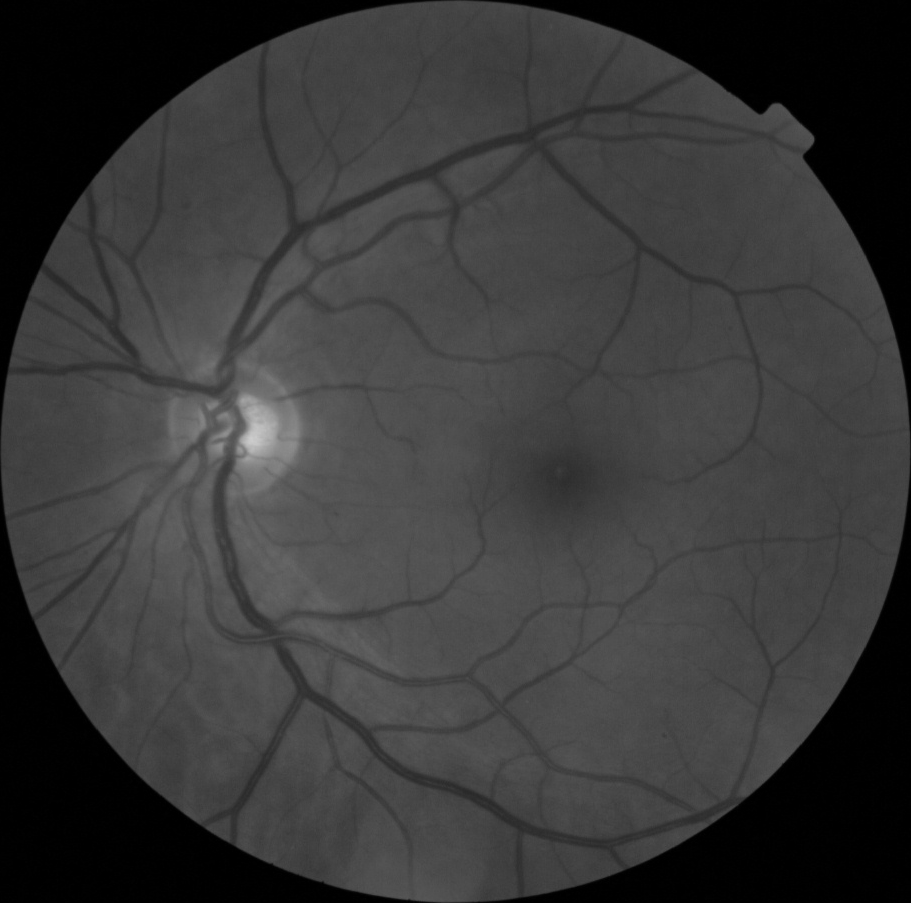
\includegraphics[width=0.5\textwidth]{saliency_gt}

      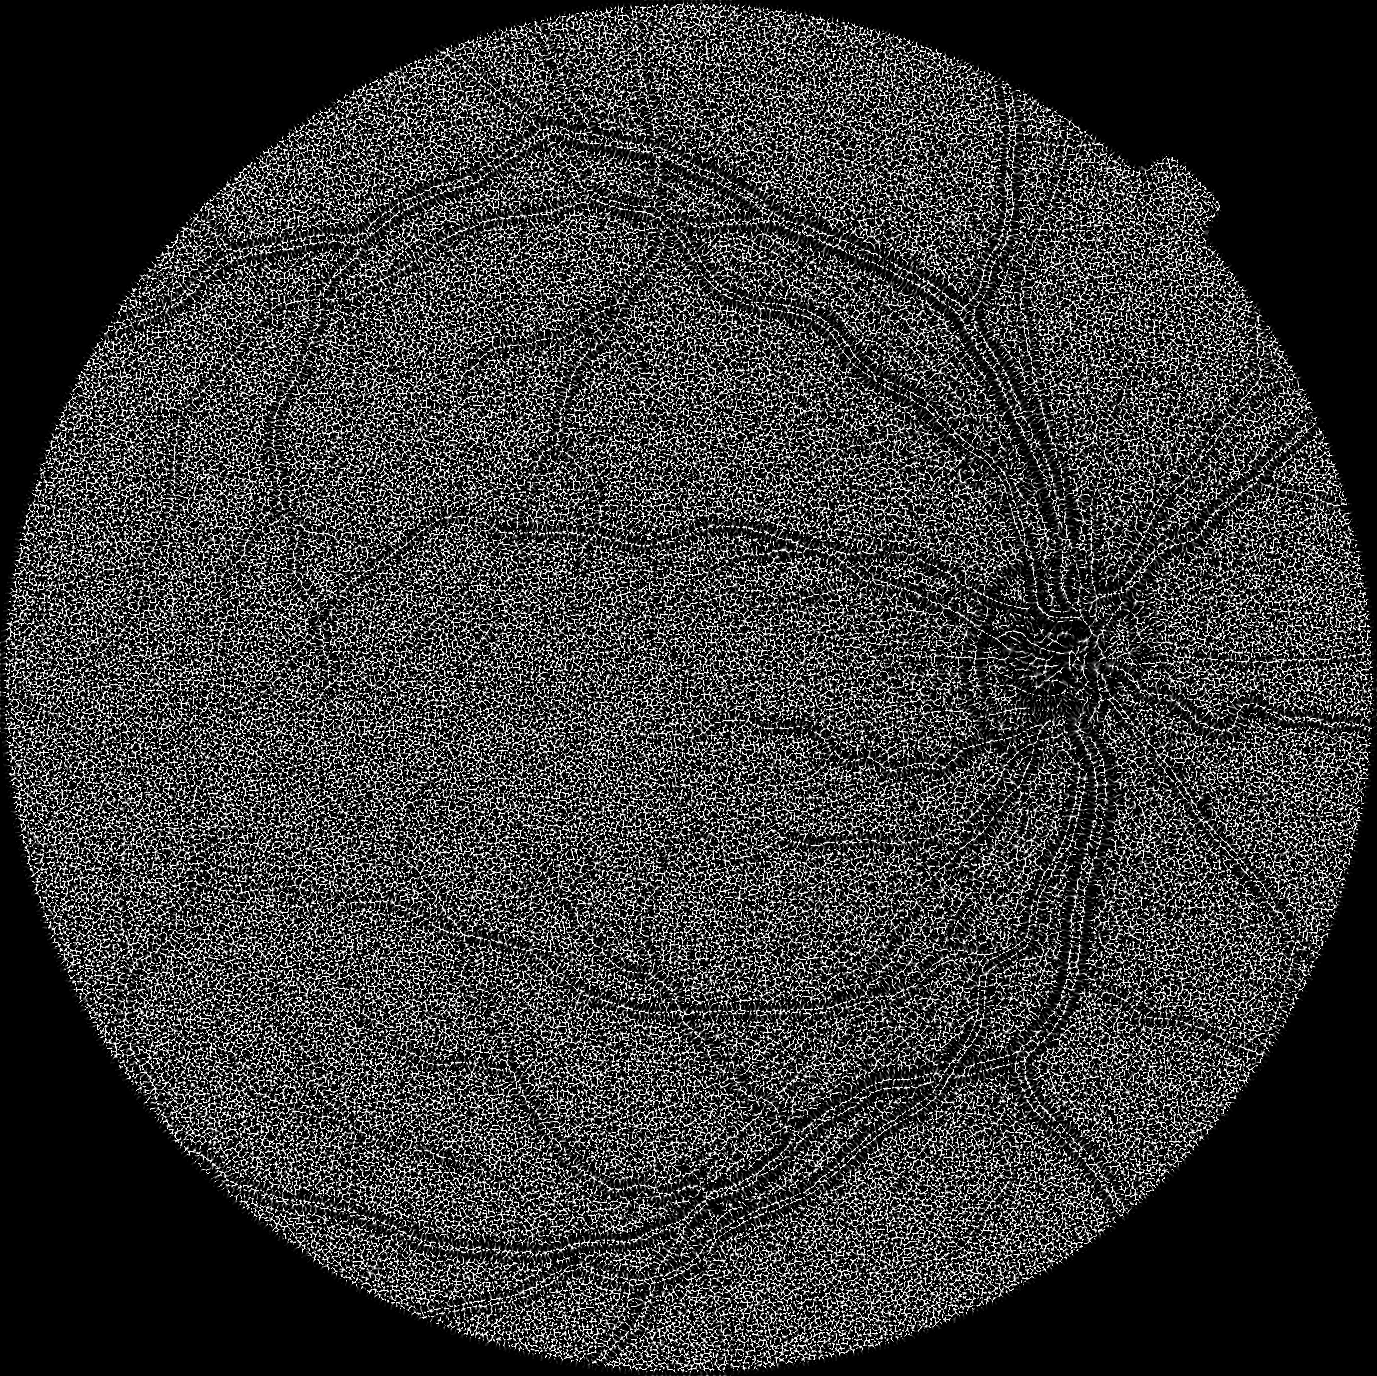
\includegraphics[width=0.8\textwidth]{saliency_vessels}
  \end{column}
  \begin{column}{0.6\linewidth}
  First component: curvature map
\begin{equation}
 I_c = \frac{\img_{xx} \img_y^2 + \img_{yy} \img_x^2 - 2 \img_{x} \img_{xy} \img_{y} }{(\img_x^2 + \img_y^2)^{1.5}}
\end{equation}
\end{column} 
\end{columns}

\end{frame}

\begin{frame}{Loss Functions 1: Saliency Weighted Charbonnier Loss (2)\footcite{SaliencyGAN}}
\begin{columns}
  \begin{column}{0.5\linewidth}
      \centering
      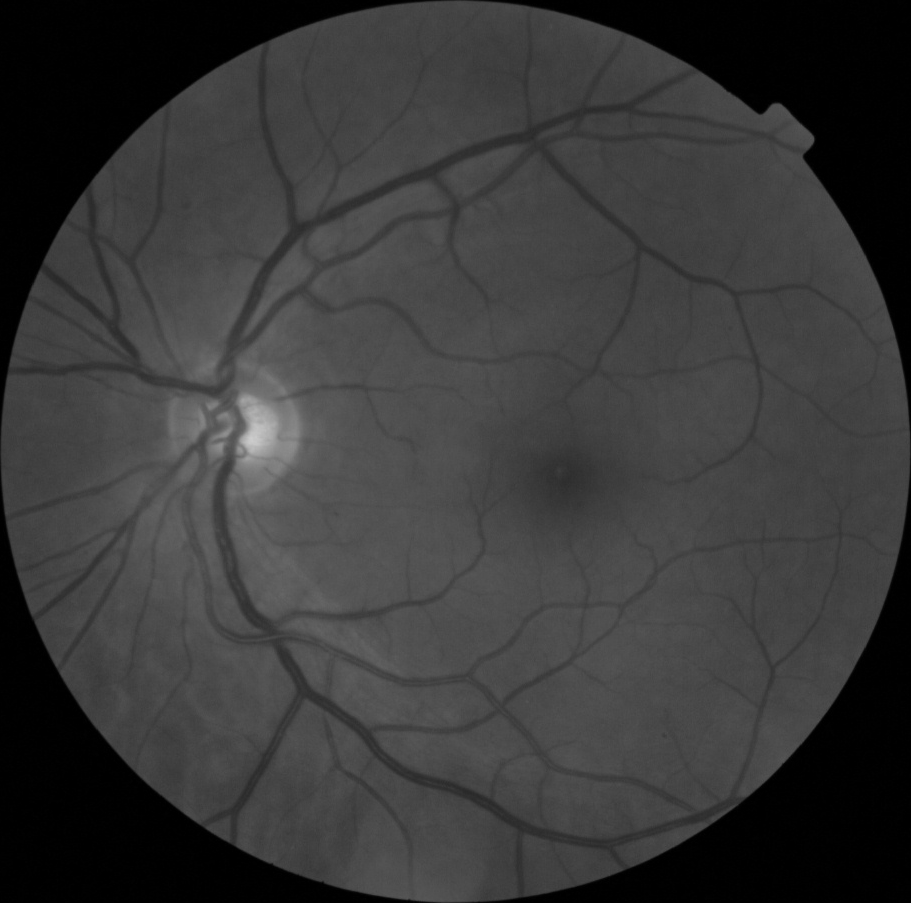
\includegraphics[width=0.5\textwidth]{saliency_gt}

      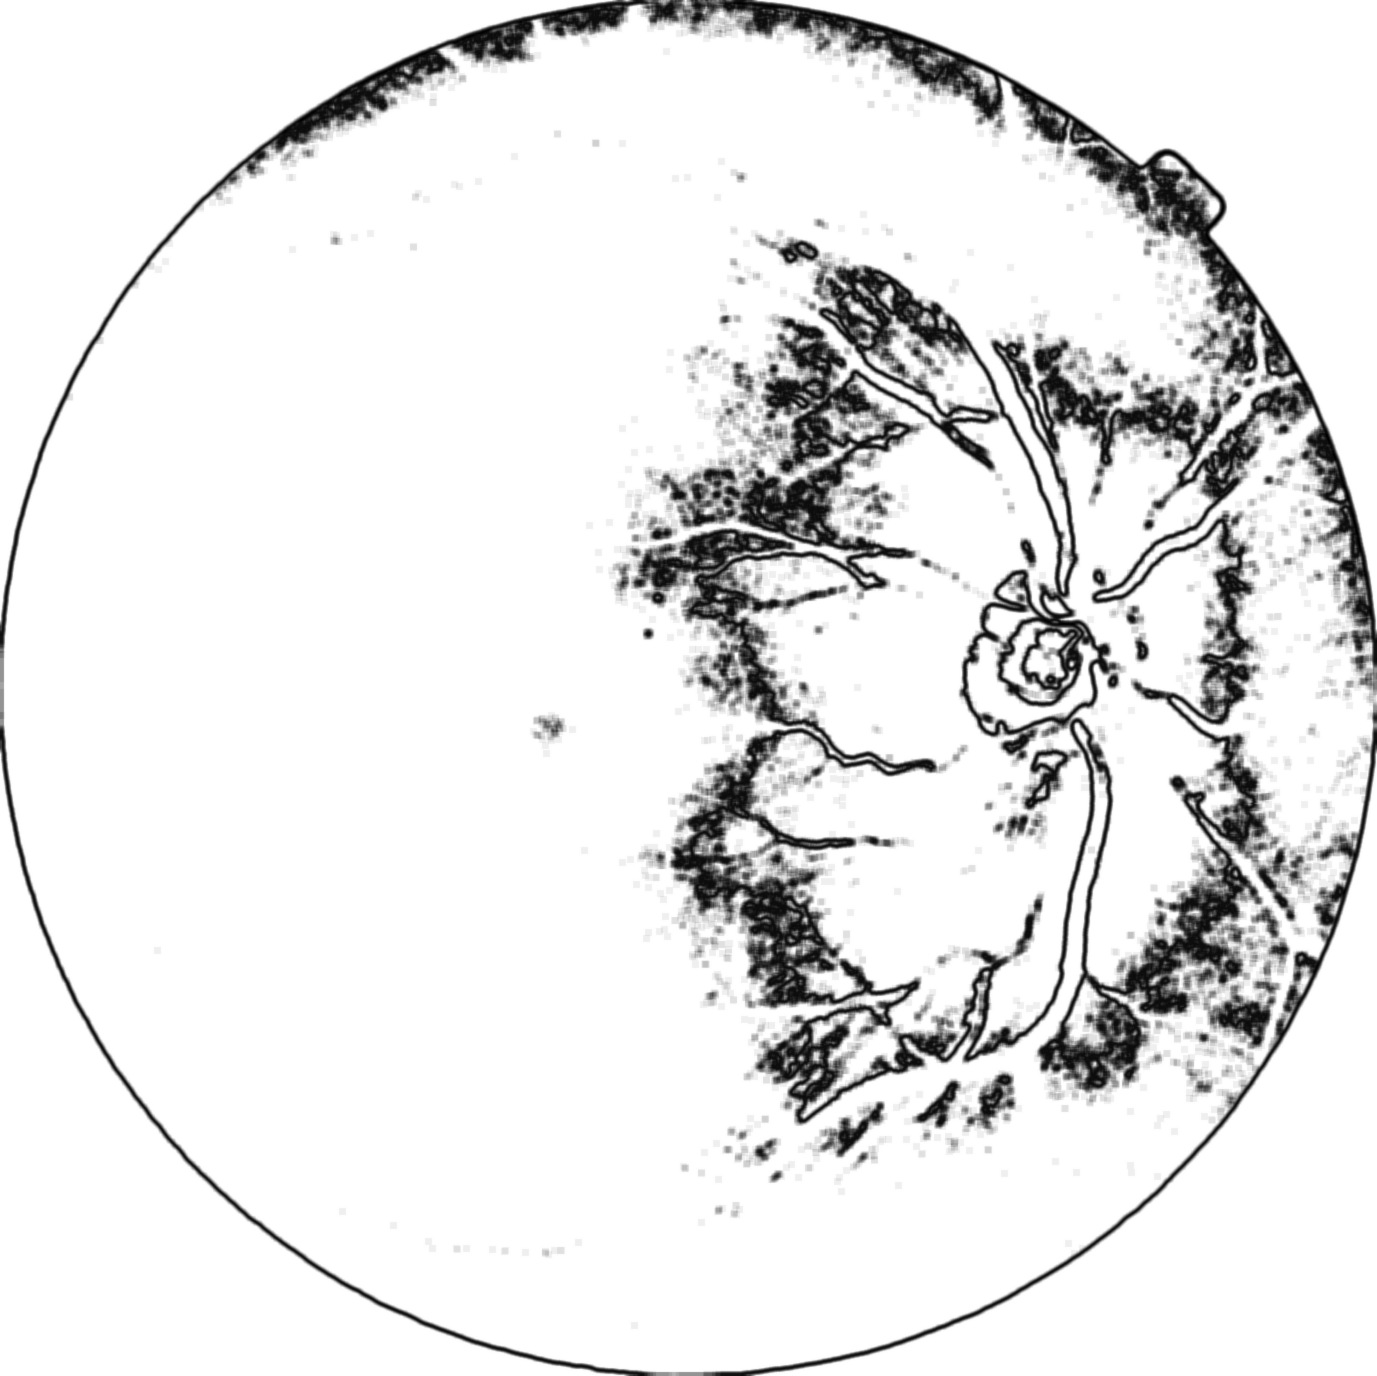
\includegraphics[width=0.8\textwidth]{saliency_entropy}
  \end{column}
  \begin{column}{0.6\linewidth}
Second component: local image entropy over $7 \times 7$ patches $P_s$ around pixel $s$
\begin{equation}
  \label{eq:entr}
  I_e = - \sum_{s \in P_s} p(s_i) \log(p(s_i)),
\end{equation}
$p(s_i)$ probability that pixel has intensity in neighborhood (approximated using histogram)

\end{column} 
\end{columns}
\end{frame}

\begin{frame}{Loss Functions 1: Saliency Weighted Charbonnier Loss (1)\footcite{SaliencyGAN}}
\begin{columns}
  \begin{column}{0.5\linewidth}
      \centering
      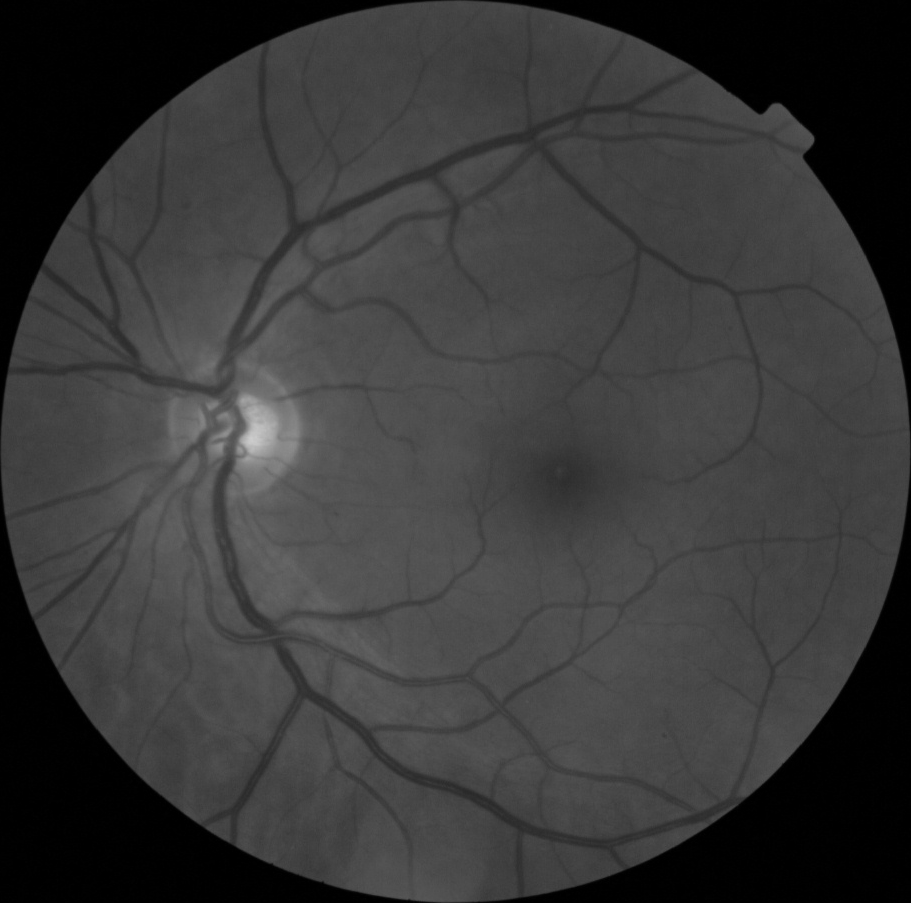
\includegraphics[width=0.5\textwidth]{saliency_gt}

      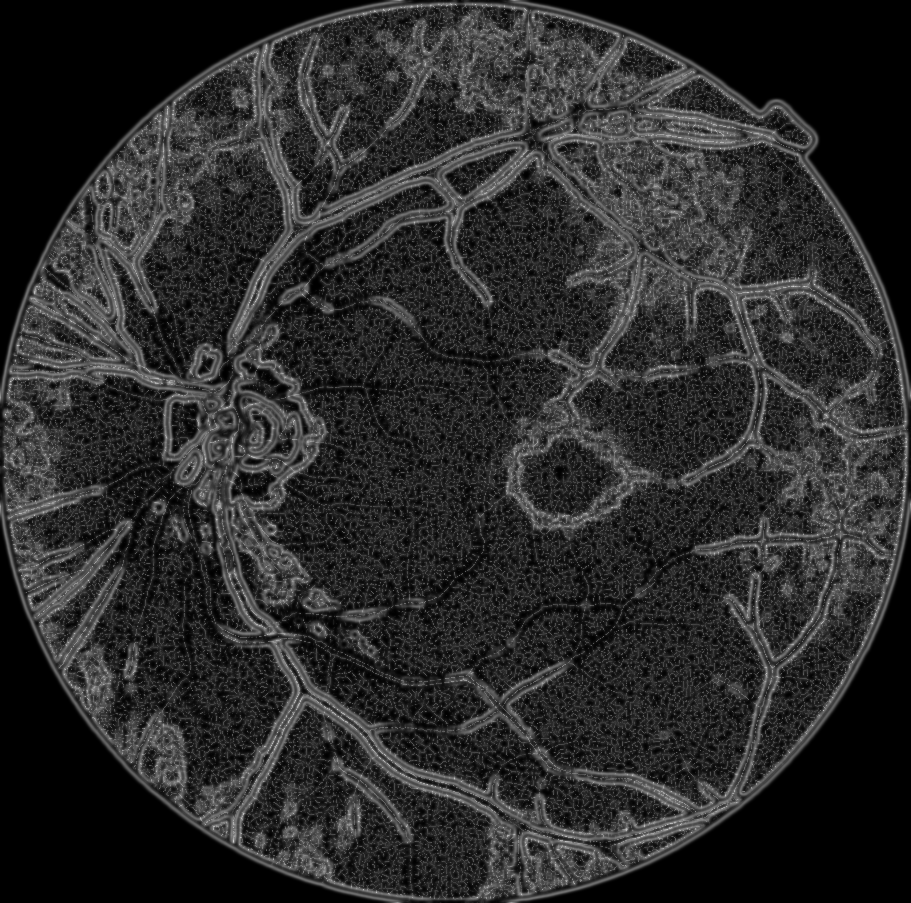
\includegraphics[width=0.8\textwidth]{saliency_full}
  \end{column}
  \begin{column}{0.6\linewidth}

Finally,
\begin{equation}
  \label{eq:saliency}
  I_{\text{sal}} = 0.4 \cdot U(I_c) + 0.6 \cdot U(1 - I_e)
\end{equation}

Linear combination of uniqueness  maps in $7 \times 7$ neighborhood
 \begin{equation}
  \label{eq:uniq}
  U(m) = \sum_{o \in P_c} w(c, o) \vert m(c) - m(o) \vert
\end{equation}
$w(c, o)$ decays exponentially for larger pixel distance between center $c$ and other $o$ 

\end{column} 
\end{columns}
\end{frame}

\begin{frame}{Loss Functions 2: Perceptual Loss\footfullcite{PerceptualLoss}}
  Compare visual features

  Filters $\phi$ taken from VGG-16 network

  First and second pooling layer got best results (correspond to low-level features)
 
\begin{equation}
  \label{eq:perceptual-loss}
  L_p(\hat{\img}, \img) = \sum_{\mathclap{l \in \{ \text{pool}_1, \text{pool}_2 \}}} \Vert \phi_l( \hat{\img} ) - \phi_l (\img) \Vert_2^2
\end{equation}
\end{frame}

\begin{frame}{Loss Function 3: Adversarial Loss\footfullcite{SRGAN}}
  Two player game between
  \begin{description}
  \item[Generator (G)] Super-resolution network
  \item[Discriminator (D)] Tries to decide, whether images are \textbf{real} high-resolution images or \textbf{generated} by our network
  \end{description}

\begin{align}
 \min_G \max_D \mathbb{E}_{\bm{x} \sim P_r} \left[ \log (D({\bm{x}})) \right] +
  \mathbb{E}_{\hat{\bm{x}} \sim P_g} \left[  \log (1 - D(\hat{\bm{x}})) \right]
\end{align}

with $P_r$ real patch distribution and $P_g$ generated patch distribution
\end{frame}

\begin{frame}{Evaluation}
  Perceptual \textit{\&} adversarial loss improve perceived quality but increase mse!

  Use:
  \begin{itemize}
  \item PSNR, pixel based
  \item SSIM\footfullcite{Ssim}, human perception based model
  \item Pixel-based error of Sobel filter (gradients)
  \item Vessel segmentation on Drive dataset\footfullcite{Drive} with retina-unet\footfullcite{RetinaUnet}
  \end{itemize}

  Compare super-resolution with bicubic interpolation \textit{\&} deblurring with an mse unet\footfullcite{Unet}.
\end{frame}

\begin{frame} \frametitle{Evaluation SR: Metrics}
\begin{table}[htb]
\centering
\caption{Results for super resolution models on Drive (Test) dataset.
  AUC corresponds to area under the ROC curve achieved by running the retina-unet on the upscaled images.
  Best results are bold.
}

\label{tab:results-sr-drive}
\begin{tabular}{@{}lS[table-format=2.2]S[table-format=2.2]S[table-format=2.2]S[table-format=2.3]@{}}
\toprule
{Model} & {PSNR} & {SSIM} & {Sobel-mse \SI{1e4}{}} & {AUC} \\ \midrule
Ground Truth & $\infty$ & 1.00 & 0.00 & 0.979 \\
Bicubic & 35.27 & 0.92 & 29.87 &  0.852 \\
Perceptual & 38.90 & 0.93 & 8.61 & 0.943 \\
Saliency & \bftabnum 39.50 & \bftabnum 0.94 & 8.55 & 0.921 \\
Saliency + Perceptual & 39.20 & 0.93 &\bftabnum 7.84 & 0.946 \\
Full & 38.85 & 0.93 & 8.29 & \bftabnum 0.948 \\
\bottomrule
\end{tabular}
\end{table}
\end{frame}

\begin{frame} \frametitle{Evaluation SR: Segmentation}
  \begin{columns}
  \begin{column}{0.33\linewidth}
      \centering
      \begin{figure}[htb]
        \centering
        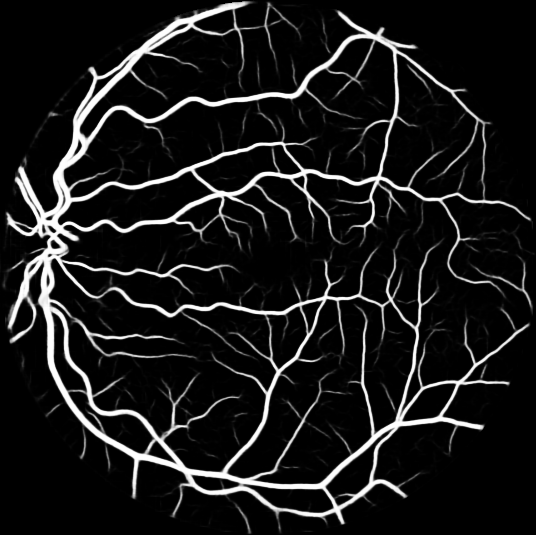
\includegraphics[width=1.0\textwidth]{segmentation_hr}
        \caption*{Segmentation HR}
      \end{figure}
    \end{column}
  \begin{column}{0.33\linewidth}
      \centering
      \begin{figure}[htb]
        \centering
        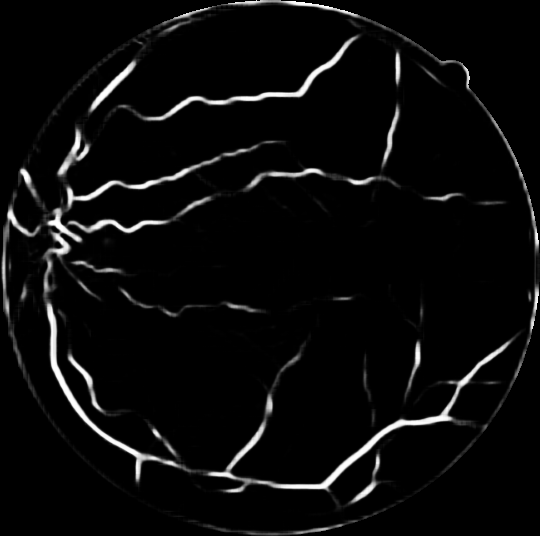
\includegraphics[width=1.0\textwidth]{segmentation_bic}
        \caption*{Segmentation Bicubic}
      \end{figure}
    \end{column}
  \begin{column}{0.33\linewidth}
      \centering
      \begin{figure}[htb]
        \centering
        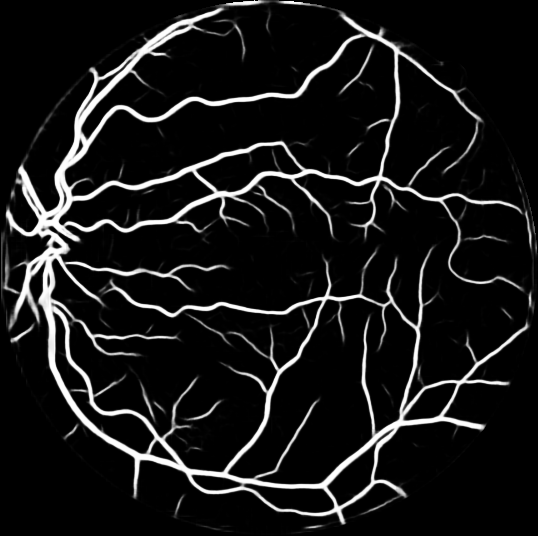
\includegraphics[width=1.0\textwidth]{segmentation_gan}
        \caption*{Segmentation SR}
      \end{figure}
    \end{column}
\end{columns}
\end{frame}

\begin{frame} \frametitle{Evaluation SR: Bicubic vs.\ Saliency }
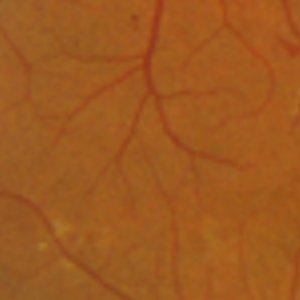
\includegraphics[width=0.48\linewidth]{patch_sr1_bic}\quad
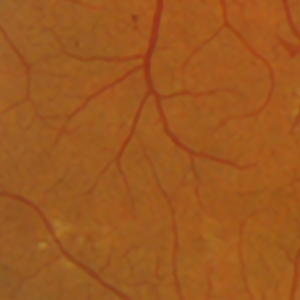
\includegraphics[width=0.48\linewidth]{patch_sr1_sal}
\end{frame}

\begin{frame} \frametitle{Evaluation SR: Saliency vs.\ Perceptual }
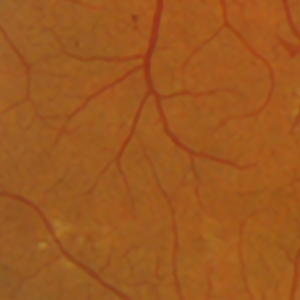
\includegraphics[width=0.48\linewidth]{patch_sr1_sal}\quad
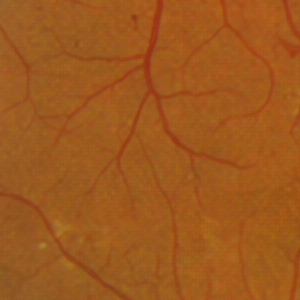
\includegraphics[width=0.48\linewidth]{patch_sr1_perc}
\end{frame}

\begin{frame} \frametitle{Evaluation SR: Perceptual vs.\ (Saliency + Perceptual) }
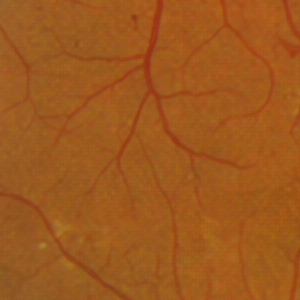
\includegraphics[width=0.48\linewidth]{patch_sr1_perc}\quad
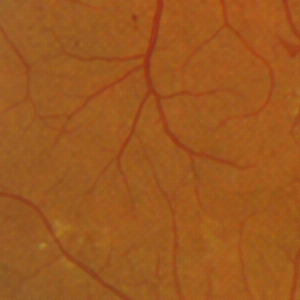
\includegraphics[width=0.48\linewidth]{patch_sr1_sal_perc}
\end{frame}

\begin{frame} \frametitle{Evaluation SR: (Saliency + Perceptual) vs.\ Full }
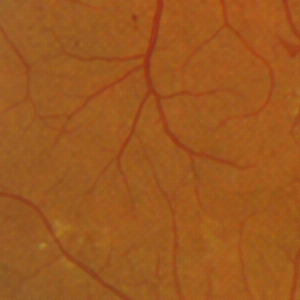
\includegraphics[width=0.48\linewidth]{patch_sr1_sal_perc}\quad
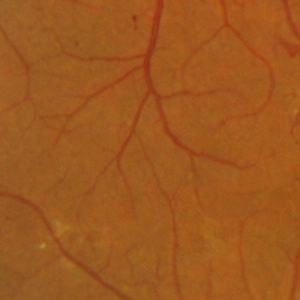
\includegraphics[width=0.48\linewidth]{patch_sr1_gan}
\end{frame}

\begin{frame} \frametitle{Evaluation SR: Full vs.\ GT }
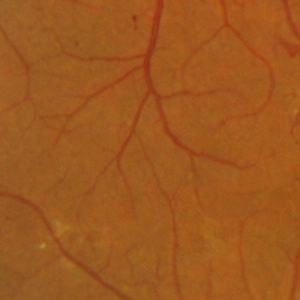
\includegraphics[width=0.48\linewidth]{patch_sr1_gan}\quad
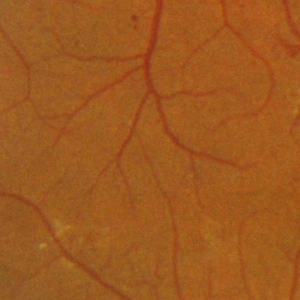
\includegraphics[width=0.48\linewidth]{patch_sr1_gt}
\end{frame}

\begin{frame} \frametitle{Evaluation SR: Artefacts (Saliency + Perceptual) }
  \centering
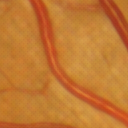
\includegraphics[width=0.7\linewidth]{patch_sr1_sal_perc_small}
\end{frame}

\begin{frame} \frametitle{Evaluation SR: Artefacts (Full) }
  \centering
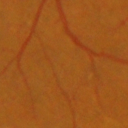
\includegraphics[width=0.7\linewidth]{patch_sr1_gan_small}
\end{frame}


\begin{frame} \frametitle{Evaluation Deblurring: Metric (Segmentation)}
  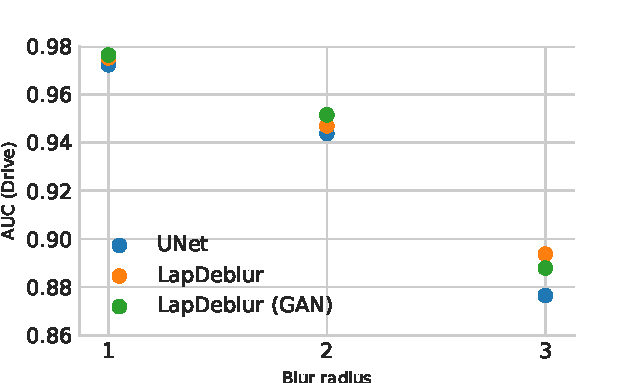
\includegraphics{deblur_auc_beamer}

  Segmentation using blurred image (radius 3): AUC of 0.654
\end{frame}

\begin{frame} \frametitle{Evaluation Deblurring: Image}
  \begin{columns}
  \begin{column}{0.33\linewidth}
      \centering
      \begin{figure}[htb]
        \centering
        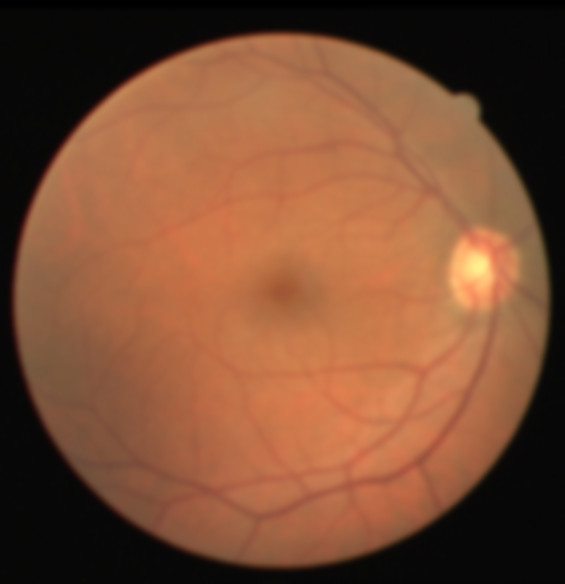
\includegraphics[width=1.0\textwidth]{deblur_lr}
        \caption*{Blur radius 3}
      \end{figure}
    \end{column}
  \begin{column}{0.33\linewidth}
      \centering
      \begin{figure}[htb]
        \centering
        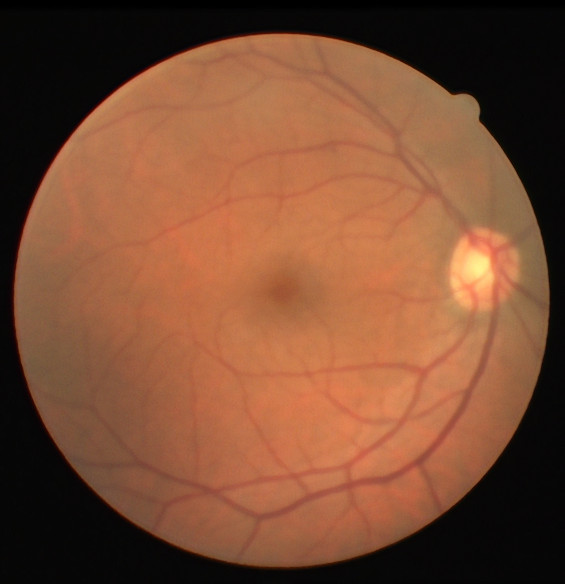
\includegraphics[width=1.0\textwidth]{deblur_gan}
        \caption*{GAN}
      \end{figure}
    \end{column}
  \begin{column}{0.33\linewidth}
      \centering
      \begin{figure}[htb]
        \centering
        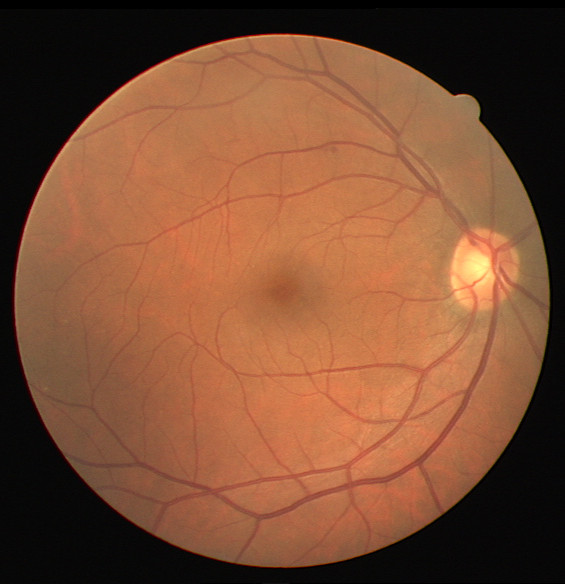
\includegraphics[width=1.0\textwidth]{deblur_gt}
        \caption*{GT}
      \end{figure}
    \end{column}
\end{columns}
\end{frame}

\begin{frame} \frametitle{Evaluation: Speed SR}
  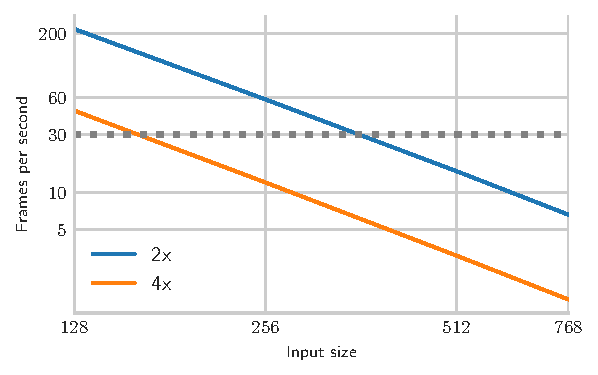
\includegraphics{time_upscaling_beamer}
\end{frame}

\begin{frame} \frametitle{Evaluation: Speed Deblurring}
  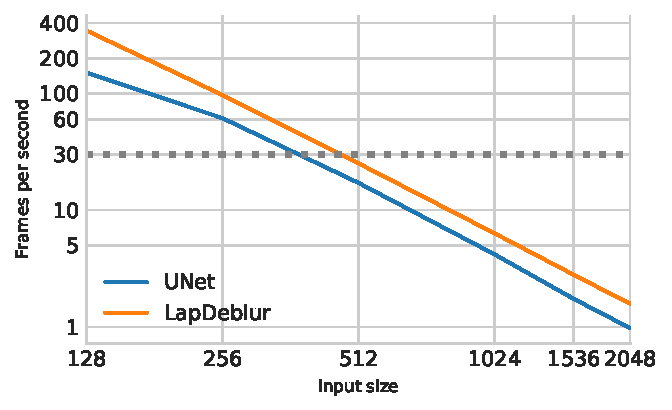
\includegraphics{time_denoising_beamer}
\end{frame}


\begin{frame}{Summary}
\begin{itemize}
  \item Solid results for both super-resolution and deblurring
  \item Usable as pre-processor
  \item Choice of loss function matters
  \item Ensemble of loss functions good compromise
  \item Real-time usage limited but possible
\end{itemize}

\centering
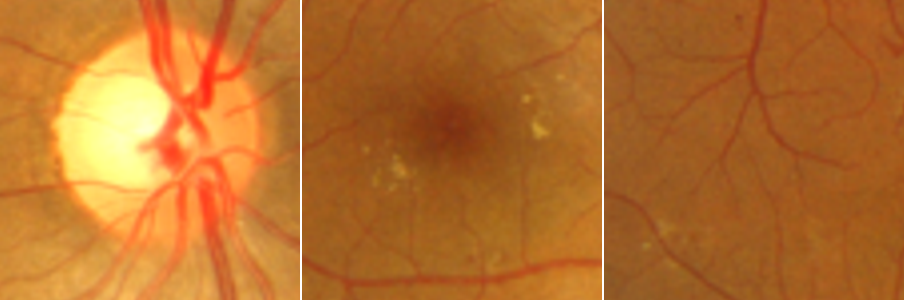
\includegraphics[width=0.6\linewidth]{collage_sr1_bic}\\
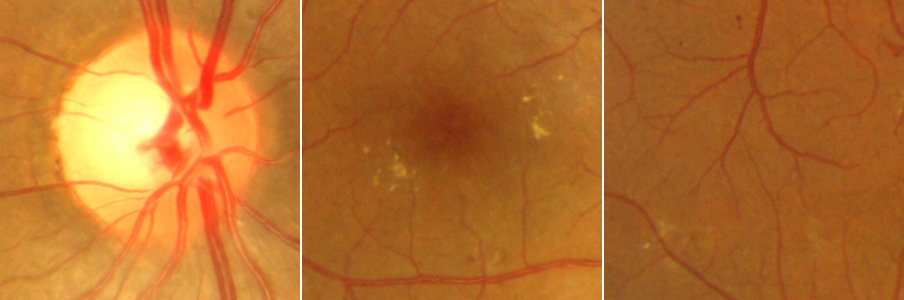
\includegraphics[width=0.6\linewidth]{collage_sr1_gan}
\end{frame}

\end{document}